Un \textbf{camino hamiltoniano} es un camino que visita cada nodo del grafo exactamente una vez. Por ejemplo, el grafo:

% TODO: \usepackage{graphicx} required
\begin{figure}[h!]
	\centering
	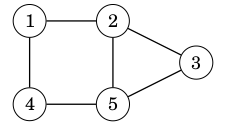
\includegraphics[width=0.3\linewidth]{img/hamilton_path}

	\label{fig:hamiltonpath}
\end{figure}


contiene una ruta hamiltoniana desde el nodo 1 al nodo 3:

\begin{figure}[h!]
	\centering
	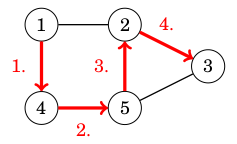
\includegraphics[width=0.3\linewidth]{img/hamilton_path_2}
	
	\label{fig:hamiltonpath2}
\end{figure}

Si un camino hamiltoniano comienza y termina en el mismo nodo, se llama \textbf{circuito o ciclo hamiltoniano}. El grafo anterior también tiene un circuito hamiltoniano que comienza
y termina en el nodo 1:

\begin{figure}[h!]
	\centering
	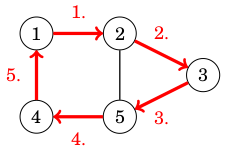
\includegraphics[width=0.3\linewidth]{img/hamilton_path_3}
	
	\label{fig:hamiltonpath3}
\end{figure}

Sobre como determinar si un grafo presenta o no un camino o ciclo de hamilton y como encontrarlo lo
veremos en esta guía.